\documentclass{article}

\usepackage[utf8]{inputenc}
\usepackage[T1]{fontenc}
\usepackage[francais]{babel}
\usepackage{url}
\usepackage{color}
\usepackage{verbatim}
\usepackage{amsmath,amssymb,amsfonts}
\usepackage{graphicx}
\usepackage[french]{algorithm2e}
\usepackage{geometry}
\usepackage{enumitem}
\usepackage{listings}
\usepackage{listingsutf8}
\frenchbsetup{StandardLists=true}
\usepackage{mcode}
\lstset{language=matlab}
\lstset{
	breaklines=true, 
	showspaces=false, 
	keepspaces=true, 
	numbers=left, 
	frame=shadowbox, 
	keywordstyle=\color{blue},
	basicstyle=\ttfamily\small,
	commentstyle=\color{green}
}
\geometry{hmargin=2.5cm, vmargin=2.5cm}

\title{Traitement d'images TP2 : Histogramme\\Segmentation d'une image, Etalement, Egalisation}
\author{Line \bsc{POUVARET}, (Hamdi \bsc{BENAOUI)}}
\date{2015-2016}

\begin{document}
\maketitle

\section*{Segmentation d’une image par seuillage des niveaux de gris}
\subsection*{1°) Algorithme de segmentation (lignes 20-75)}

Cet algorithme correspond à l’algorithme des K-Moyennes. Il va itérer maximum 200 fois afin de trouver les seuils de niveau de gris de l’image qu’on choisit pour segmenter l’image par la suite. A partir de l’histogramme des niveaux de gris des pixels de l’image,  on arrive à séparer les groupes de pixels ayant sensiblement le même niveau de gris et ces séparations vont constituer nos seuils.

\subsection*{2°) Instructions ajoutées dans le programme}
\begin{lstlisting}
Pour le mode 'thres' :
level =(v_threshold(k) + v_threshold(k+1))/2;

Pour le mode 'mean' :
if(N(k)~=0)
                current_X = [v_threshold(k):v_threshold(k+1)-1]';
                h2=histo(current_X+1);
                level = h2'*current_X/N(k);
            else
                level = 0; 
\end{lstlisting}

\subsection*{3°)} 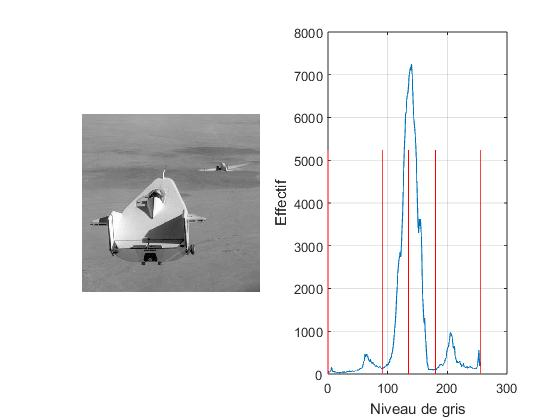
\includegraphics[width=8cm]{liftingbody_avant.jpg}

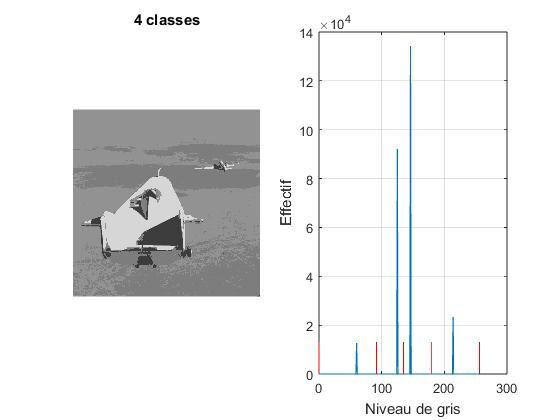
\includegraphics[width=8cm]{liftingbody_4classes.jpg}
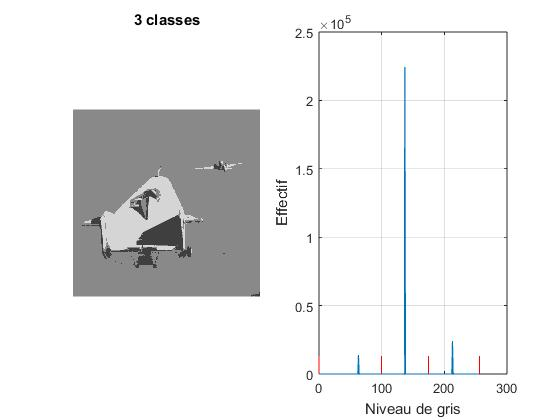
\includegraphics[width=8cm]{liftingbody_3classes.jpg}
\subsection*{4°) Instructions ajoutées dans le programme}
\begin{lstlisting}
[nbMax,classeMax] = max(seg_histo(:));
map = gray(256);
map(classeMax,:) = [1 0 0];
 
figure
colormap(map);
subplot(1,2,1)
image(segmented_pic)
axis equal
axis off
title([int2str(nbr_class) ' classes'])
subplot(1,2,2)
plot(seg_bin,seg_histo);
hold on
for k = 1 : length(v_threshold)
    plot(v_threshold(k)*[1 1], [0 nbpix/20], 'r-')
end
grid on
xlabel('Niveau de gris')
ylabel('Effectif')
 
figure(n1)
subplot(1,2,2)
hold on
for k = 1 : length(v_threshold)
    plot(v_threshold(k)*[1 1], [0 nbpix/50], 'r-')
end
\end{lstlisting}

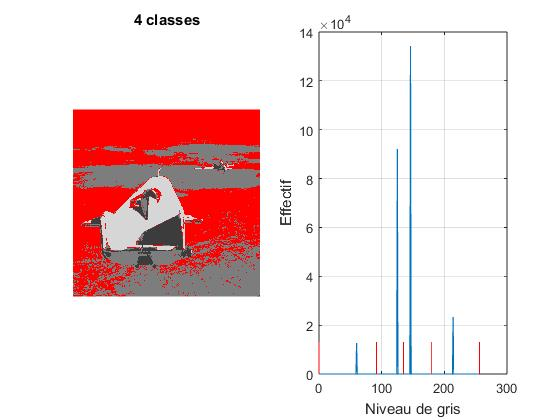
\includegraphics[width=8cm]{liftingbody_rouge.jpg}

\subsection*{5°) }

\section*{Modification d’histogramme sur une image en noir et blanc}
\subsection*{A°) Etalement d’un histogramme de niveaux de gris}
\begin{enumerate}[label=\arabic*$\degres$)]
	\item Cet appel permet de générer un histogramme à partir d’une image et d’un nombre de couleurs (niveaux de gris ici). h correspond à la hauteur des barres, et n l’indice des barres de l’histogramme. L’histogramme représente le nombre de pixels par niveau de gris.
	\item Instructions ajoutées dans la fonction histo\_etalement :
\begin{lstlisting}
pic = 255*((original_pic-pic_min)/(pic_max-pic_min));
pic = uint8(max(min(pic,255),0));
\end{lstlisting}

\end{enumerate}
On remarque sur l’histogramme qu’on a un peu plus étalé nos niveaux de gris entre 0 et 255.

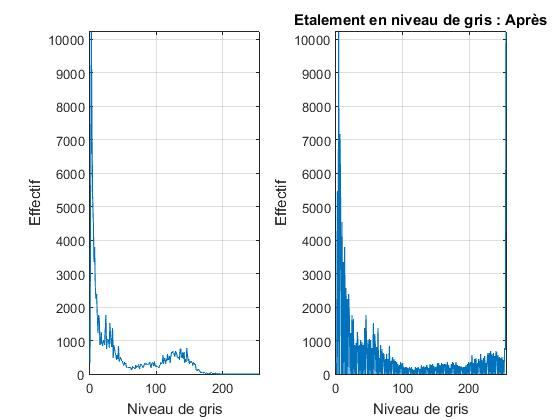
\includegraphics[width=10cm]{Venise_histo_etalement.jpg}

\begin{enumerate}[label=\arabic*$\degres$)]
	\item 
	\begin{itemize}\renewcommand{\labelitemi}{$\bullet$}
		\item Quand on met factor\_min et factor\_max à 1 tous les deux, on obtient l’image d’origine comme image de sortie et les deux histogrammes sont les mêmes (donc on n’a pas eu d’étalement).
		\item Quand on met factor\_min et factor\_max à 0.5 tous les deux, on obtient une image très sombre et l’histogramme de sortie est compressé vers les niveaux de gris sombres.
		\item Factor\_max=1, factor\_min=0 $\rightarrow$ image de sortie = image d’origine
		\item Plus on augmente sensiblement la valeur de factor\_max (>1) plus on va étaler nos pixels et les éloigner des nuances très sombres.
		\item Dès que factor\_max < 1, on compresse les pixels vers les niveaux de gris plus sombres.
	\end{itemize}
	\item L'image d’origine est globalement très sombre au départ. La majorité des pixels se situe dans les niveaux de gris sombres mais il y a un certain nombre de pixels proches de nuances plus claires (ceux qui constituent les nuances du ciel).

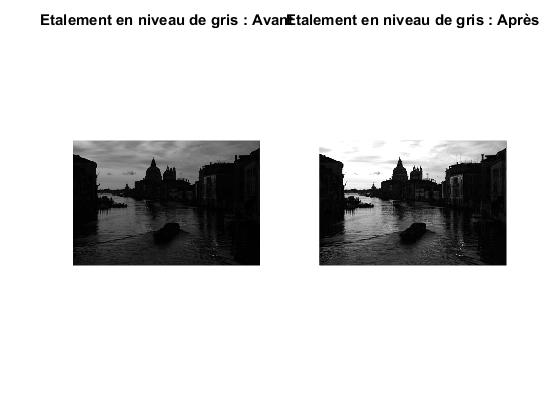
\includegraphics[width=10cm]{Venise_etalement.jpg}

Quand on va augmenter notre alpha (factor\_max), > 1, on étale les pixels beaucoup plus vers les niveaux de gris sombres.
Si on augmente trop alpha, on aura tendance à avoir une image beaucoup trop claire. Il faudrait arriver à étaler énormément pour les pixels très nombreux des nuances sombres et étaler moins pour les nuances claires (sinon le ciel apparaît beaucoup trop blanc).
\end{enumerate}

\subsection*{B°) Egalisation d’histogramme de niveaux de gris}
\begin{enumerate}[label=\arabic*$\degres$)]
\lstset{frame=none, numbers = none}
	\item
	\begin{lstlisting}
lut = 255/nbr\_pixels*cumsum(old\_histo);
\end{lstlisting}

C’est cette ligne de code qui permet de calculer notre fonction de transformation. 

$\phi$($n_{e}$) = ($N_{max}$ / NT) * $ch_{e}$($n_{e}$)
Avec : \begin{itemize}\renewcommand{\labelitemi}{$\bullet$}
		\item $\phi$($n_{e}$) = lut $\rightarrow$ la fonction de transformation
		\item $N_{max}$ = 255 $\rightarrow$ Niveaux de gris max dans l’image
		\item NT=nbr\_pixels $\rightarrow$ nombre de pixels total
		\item $ch_{e}$($n_{e}$ = cumsum(old\_histo) $\rightarrow$ cumul de l’histogramme

La suite de la fonction permet de reshape l’image avec la fonction de transformation lut et on reconvertit en int.
 	\end{itemize}
	\item On voit que sur l'image, on a énormément diminué le contraste entre les nuances sombres et les nuances claires. L'image est globalement plus composée de nuances moyennes.

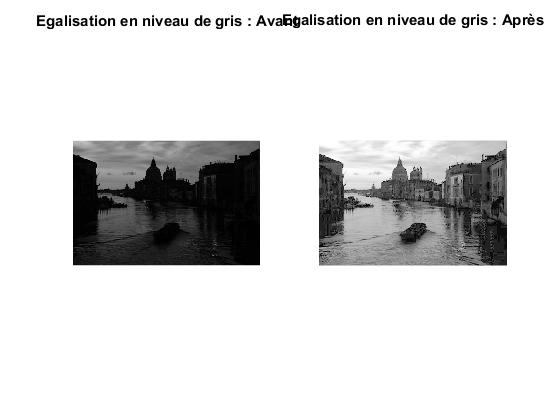
\includegraphics[width=10cm]{Venise_egalisation.jpg}

On constate bien que sur l'histogramme, les valeurs des pixels sont plus proches du centre qu'avant. On a essayé d'égaliser la répartition des pixels sur l'histogramme.\\

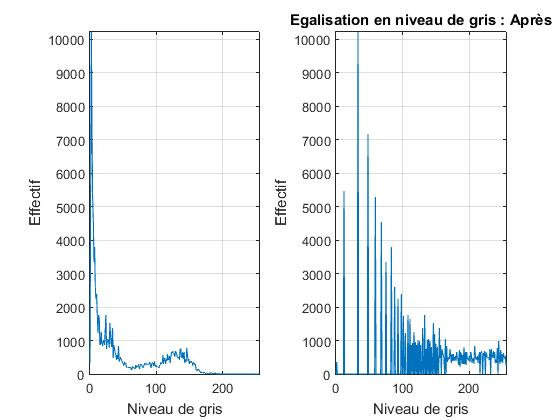
\includegraphics[width=10cm]{Venise_histo_egalisation.jpg}

	\item On remarque que les parties qui étaient les plus sombres sur l'image sont devenues, après égalisation, moins précises.

On a perdu de l'information au niveau du détail et cela forme des paquets de pixels incohérents à certains endroits (notamment en bas à gauche).\\
\end{enumerate}

\section*{Modification d’histogramme sur une image en couleurs, approche naïve}
\subsection*{\underline{C°) Etalement d’histogramme de couleurs}}
\begin{enumerate}[label=\arabic*$\degres$)]
	\lstset{numbers=left, frame=shadowbox} 
	\item Instructions ajoutées au programme :

\begin{lstlisting}
[pic_RGB_linearized,h_r,h_r0] = histo_etalement(pic(:,:,1),factor_max,factor_min);
[pic_RGB_linearized,h_g,h_g0] = histo_etalement(pic(:,:,2),factor_max,factor_min);
[pic_RGB_linearized,h_b,h_b0] = histo_etalement(pic(:,:,3),factor_max,factor_min);
\end{lstlisting}

On obtient les résultats suivants :

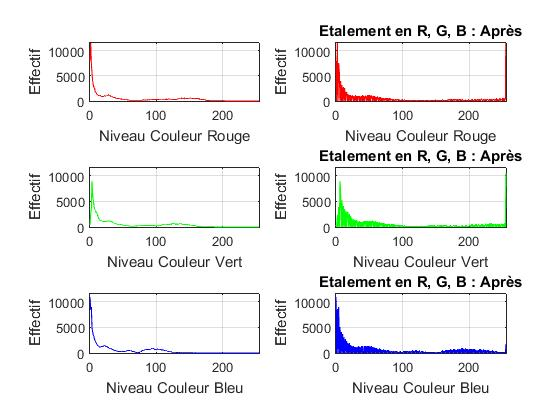
\includegraphics[width=8cm]{Venise_RGB_histo_etalement.jpg}
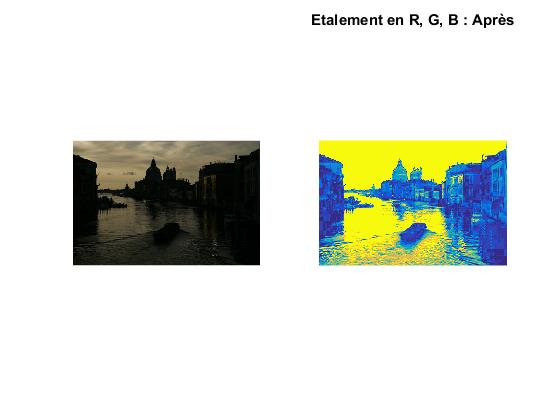
\includegraphics[width=8cm]{Venise_RGB_etalement.jpg}

On a généré de fausses couleurs en voulant étirer nos histogrammes de chaque composante. (Puisque chaque histogramme est différent)
	\item En faisant varier les facteurs alpha et beta, on constate que les nuances sombres vont soit se rapprocher du bleu soit s'en séloigner et les nuances claires vont soit s'approcher du jaune soit s'en éloigner.
\end{enumerate}

\subsection*{\underline{D°) Egalisation d’histogramme de couleurs}}
\begin{enumerate}[label=\arabic*$\degres$)]
	\item Instructions ajoutées au programme :

\begin{lstlisting}
[pic_RGB_equalized,h_r,h_r0] = histo_egalisation(pic(:,:,1));
[pic_RGB_equalized,h_g,h_g0] = histo_egalisation(pic(:,:,2));
[pic_RGB_equalized,h_b,h_b0] = histo_egalisation(pic(:,:,3));
\end{lstlisting}

On obtient les résultats suivants :

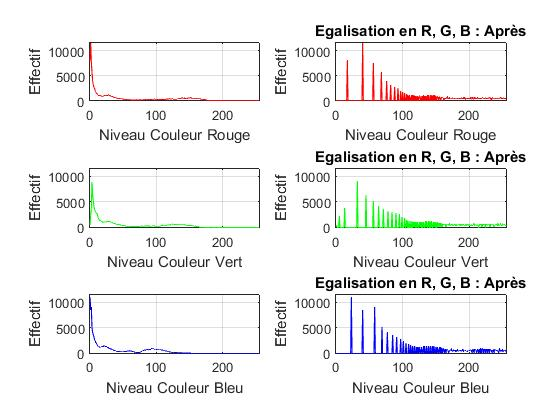
\includegraphics[width=8cm]{Venise_RGB_histo_egalisation}
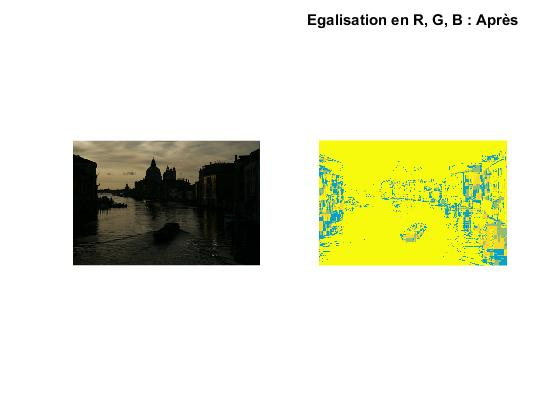
\includegraphics[width=8cm]{Venise_RGB_egalisation}

	\item L'image de Venise est devenue pratiquement entièrement jaune, les pixels ont tous été rapprochés vers la même nuance de couleur (ici le jaune).
On voit bien sur les histogrammes que les pixels sont répartis de manière plus uniforme et plus vers des valeurs moyennes.
\end{enumerate}

\section*{Changement de base « couleur » (NON FINI)}
\subsection*{\underline{E°)}}
\begin{enumerate}[label=\arabic*$\degres$)]
	\item Plus une couleur va contenir du rouge et plus Cr va être positive. Plus elle va contenir du vert, plus elle va avoir une valeur négative.

Une couleur jaune a un Cr de 0. Une couleur rouge aura un Cr maximum et une couleur verte aura un Cr minimum.

Cb code l'opposition de couleur bleu-jaune.

Cr code l'opposition de couleur rouge-vert.
	\item \begin{itemize}\renewcommand{\labelitemi}{$\bullet$}
		\item instructions ajoutées à la fonction convert\_RGB\_to\_YCbCr :

\begin{lstlisting}
pic_YCbCr = reshape(double(pic_rgb)./255,[],3)*M;
pic_YCbCr = reshape(pic_YCbCr,size(pic_rgb));
\end{lstlisting}

		\item instructions ajoutées à la fonction convert\_YCbCr\_to\_RGB :
\begin{lstlisting}
M = [ [ 0.299 , 0.587 , 0.114];...
      [-0.168 ,-0.331 , 0.5];...
      [ 0.5 ,-0.4187 ,-0.0813] ];
  
pic_rgb = reshape(double(pic_YCbCr), [], 3)*inv(M);
pic_rgb = reshape(pic_rgb, size(pic_YCbCr));

pic_rgb = pic_rgb.*255;
pic_rgb = uint8(pic_rgb);
\end{lstlisting}
	\end{itemize}
\end{enumerate}

\section*{Etalement d’histogramme de couleurs (YCbCr)}
\subsection*{\underline{F°)}}
\begin{enumerate}[label=\arabic*$\degres$)]
	\item Instructions ajoutées dans le programme :
\begin{lstlisting}
pic_Lum_linearized = uint8(zeros(size(pic)));
pic_Lum_linearized=convert_rgb_to_YCbCr(pic);
[pic_Lum_linearized_Y,h,h0] = histo_etalement(pic_Lum_linearized(:,:,1),factor_max,factor_min);
pic_Lum_linearized(:,:,1) = double(pic_Lum_linearized_Y)./255;
pic_Lum_linearized = convert_YCbCr_to_rgb(pic_Lum_linearized);
\end{lstlisting}
\end{enumerate}

\section*{Egalisation d’histogramme de couleurs (YCbCr)}
\subsection*{\underline{G°)}}

\begin{enumerate}[label=\arabic*$\degres$)]
	\item Instructions ajoutées dans le programme :
\begin{lstlisting}
pic_Lum_equalized = uint8(zeros(size(pic)));
pic_Lum_equalized = convert_rgb_to_YCbCr(pic);
[pic_Lum_equalized_Y,h,h0] = histo_egalisation(pic_Lum_equalized(:,:,1));
pic_Lum_equalized(:,:,1) = double(pic_Lum_equalized_Y)./255;
pic_Lum_equalized = convert_YCbCr_to_rgb(pic_Lum_equalized);
\end{lstlisting}
\end{enumerate}

\end{document}